% @Author: Luis Perez
% @Date:   2016-02-02 21:09:55
% @Last Modified by:   luis
% @Last Modified time: 2016-02-19 17:47:15

\documentclass[12pt]{article}
\usepackage{latexsym}
\usepackage{fancyhdr}
\usepackage{amssymb,amsmath,amsthm}
\usepackage[pdftex]{graphicx}
\usepackage{pdfpages}
\usepackage{hyperref}
\usepackage[margin=1in]{geometry}


% Create answer counter to keep track of seperate responses
\newcounter{AnswerCounter}
\newcounter{SubAnswerCounter}
\newcounter{SubSubAnswerCounter}
\setcounter{AnswerCounter}{1}
\setcounter{SubAnswerCounter}{1}
\setcounter{SubSubAnswerCounter}{1}

% Create answer environment which uses counter
\newenvironment{answer}[0]{
  \setcounter{SubAnswerCounter}{1}
  \bigskip
  \textbf{Solution \arabic{AnswerCounter}}
  \\
  \begin{small}
}{
  \end{small}
  \stepcounter{AnswerCounter}
}

\newenvironment{subanswer}[0]{
  \setcounter{SubSubAnswerCounter}{1}
  (\alph{SubAnswerCounter})
}{
 \bigskip
  \stepcounter{SubAnswerCounter}
}

\newenvironment{subsubanswer}[0]{
  \hspace{0.25in}[\roman{SubSubAnswerCounter}]
}{
 \bigskip
  \stepcounter{SubSubAnswerCounter}
}

% Allows easy use of vectors
\newcommand{\vect}[1]{\vec{\boldsymbol{#1}}}


% Custom Header information on each page
\pagestyle{fancy}
\lhead{HUID: 70871564}
\rhead{Luis Perez - \thepage}
\renewcommand{\headrulewidth}{0.1pt}
\renewcommand{\footrulewidth}{0.1pt}

\newcommand{\horrule}[1]{\rule{\linewidth}{#1}}   % Horizontal rule

\title{
    % \vspace{-1in}
    \usefont{OT1}{bch}{b}{n}
    \normalfont \normalsize \textsc{Harvard University} \\ [25pt]
    \horrule{0.5pt} \\[0.4cm]
    \huge Physics 143a: Quantum Mechanics I \\ [20pt]
    \normalfont \normalsize Problem Set 3
    \horrule{2pt} \\[0.5cm]
}
\author{
    \normalfont                 \normalsize
        Luis Antonio Perez\\[-3pt]    \normalsize
}
\date{\today}

\begin{document}
\maketitle
\pagebreak


\begin{answer}
\begin{subanswer}
The stationary states of an isolated system do not change with time. In fact, we can formally show that the probability distribution associated with stationary state $\psi$, given by $|\psi|^2$, is not dependent on time $t$. Additionally, in a stationary state, all measurements (expectation values) are constants. Furthermore, the stationary states are of importance because all wave function $\Psi(x,t)$ can be written as a linear combination of the stationary states $\Psi(x)$ as follows:
$$
\Psi(x,t) = \sum_{n=1}^{\infty} c_n \psi(x)e^{-iE_nt / \hbar}
$$
\end{subanswer}

\begin{subanswer}
We consider a particle in the first excited state of an infinite square well system (``particle in a box''). Note that the solutions to the SE is given as:
$$
\Psi(x,t)_2 = \sqrt{\frac{2}{a}}\sin\left( \frac{2\pi}{a}x\right)e^{-iE_2t / \hbar}
$$
where $a$ is the length of the well and $E_n = n^2 \frac{\hbar^2\pi^2}{2ma^2}$ so that we have the probability density as:
$$
|\Psi(x,t)_2|^2 = \frac{2}{a}\sin^2\left(\frac{2\pi}{a}x \right)
$$
\begin{subsubanswer}
The plot of the above is presented in Figure \ref{fig:infinite_well_2}, where we fix $a = 2$ (width).
\begin{figure}[h!]
\centering
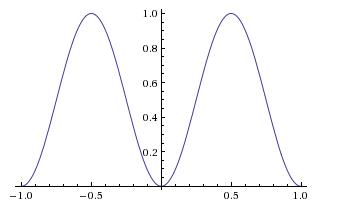
\includegraphics{infinite_well_n=2.jpg}
\caption{Probability density distribution for an infinite square well with boundaries at $x = -1$ and $x = 1$ for the
first excited state.}
\label{fig:infinite_well_2}
\end{figure}
\end{subsubanswer}

\begin{subsubanswer}
We now consider the average value of the position operator.

\begin{align}
  \langle x \rangle &= \int_{-a/2}^{a/2} x |\Psi(x,t)|^2 dx \\
  &= \frac{2}{a} \int_{-a/2}^{a/2} x \sin^2\left(\frac{2\pi}{a}x \right) \\
  &= 0
\end{align}

Note that in the last step we take notice that the function we're integrating is odd, and therefore the integral from $-a/2$ to $a/2$ is $0$.
\end{subsubanswer}

\begin{subsubanswer}
Neither of the above values depend on time because this is a stationary state. We can see this directly from the fact that the time dependence cancels out when computing $|\Psi(x,t)_2|$. Figure \ref{sketch_1} shows the sketches.

\begin{figure}[h!]
\centering

\includegraphics[scale=0.5]{blank.png}

\includegraphics[scale=0.5]{blank.png}
\caption{(Left) Sketch of position measurements as time passes. (Right) Sketch of the probability density as time passes}
\label{sketch_1}
\end{figure}
\end{subsubanswer}
\end{subanswer}

\begin{subanswer}
We now consider a particle in the second excited state. Note that the SE solution is given as:
$$
\Psi_3(x,t) = \sqrt{\frac{2}{a}} \cos\left(\frac{3\pi}{a}x\right)e^{-iE_3t / \hbar}
$$
where $a$ is the length of the well and $E_n$ is as defined before. Then the probability density is given by:
$$
|\Psi_3(x,t)|^2 = \frac{2}{a} \cos^2\left(\frac{3\pi}{a}x \right)
$$
\begin{subsubanswer}
The plot of the above is presented in Figure \ref{fig:infinite_well_3} where we fix $a=2$ (width).
\begin{figure}[h!]
\centering
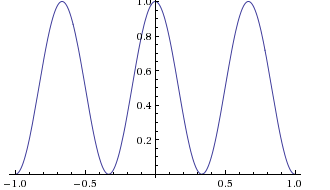
\includegraphics{infinite_well_3.png}
\caption{Probability density distribution for an infinite square well with boundaries at $x = -1$ and $x = 1$ for the
second excited state.}
\label{fig:infinite_well_3}
\end{figure}
\end{subsubanswer}
\begin{subsubanswer}
We now consider the value of the position operator.
\begin{align}
  \langle x \rangle &= \int_{-a/2}^{a/2} x |\Psi_3(x,t)|^2 dx \\
  &= \frac{2}{a} \int_{-a/2}^{a/2} x \cos^2\left(\frac{3\pi}{a}x \right) \\
  &= 0
\end{align}
where we used the fact that the integrand is an odd function.
\end{subsubanswer}

\begin{subsubanswer}
Neither of the above values depend on time because this is a stationary state. Figure \ref{sketch_2} shows the sketches.

\begin{figure}[h!]
\centering

\includegraphics[scale=0.5]{blank.png}

\includegraphics[scale=0.5]{blank.png}
\caption{(Left) Sketch of position measurements as time passes. (Right) Sketch of the probability density as time passes}
\label{sketch_2}
\end{figure}

\end{subsubanswer}
\end{subanswer}

\begin{subanswer}
We now consider a particle in a superposition of the first two excited states, $\Psi_3(x,t)$ and $\Psi_2(x,t)$. Therefore, the wave function is given by:
$$
\Psi(x,t) = c_2 \Psi_2(x,t) + c_3 \Psi_3(x,t)
$$

\begin{subsubanswer}
We now normalize $\Psi(x,t)$.
\begin{align*}
\int_{-a/2}^{a/2} |\Psi(x,t)|^2 dx &= \int_{-a/2}^{a/2} \Psi^*(x,t)\Psi(x,t) dx \\
&= \int_{-a/2}^{a/2} [c_2^* \Psi_2^*(x,t) + c_3^* \Psi_3^*(x,t)][c_2 \Psi_2(x,t) + c_3 \Psi_3(x,t)] dx \\
&= |c_2|^2 + |c_3|^2
\end{align*}
Given that the given state implies that the two wave stationary states are mixed by equal parts, we have that the normalized wave function is given by:
$$
\Psi(x,t) = \frac{1}{\sqrt{2}}\Psi_2(x,t) + \frac{1}{\sqrt{2}}\Psi_3(x,t)
$$
\end{subsubanswer}

\begin{subsubanswer}
The probability is then given by:
\begin{align*}
|\Psi(x,t)|^2 &= [c_2^*\Psi_2^*(x,t) + c_3^*\Psi_3^*(x,t)]\cdot[c_2\Psi_2(x,t) + c_3\Psi_3(x,t)] \\
&= |c_2|^2|\Psi_2(x,t)|^2 + |c_3|^2|\Psi_3(x,t)|^2 + c_2^*c_3\Psi_2^*(x,t)\Psi_3(x,t) + c_2c_3^* \Psi_3^*(x,t)\Psi_2(x,t) \\
&= \frac{1}{a}\sin^2\left(\frac{2\pi}{a}x \right) +  \frac{1}{a} \cos^2\left(\frac{3\pi}{a}x \right) + \frac{1}{a} \sin\left(\frac{2\pi}{a}x \right) \cos\left(\frac{3\pi}{a}x \right)e^{i[E_2 - E_3]t / \hbar} \\
&+ \frac{1}{a}\sin\left(\frac{2\pi}{a}x \right) \cos\left(\frac{3\pi}{a}x \right)e^{i[E_3 - E_2]t / \hbar}\\
&= \frac{1}{a}\left[ \sin^2\left(\frac{2\pi}{a}x \right) + \cos^2\left(\frac{3\pi}{a}x \right) + \left[ e^{-i[E_3 - E_2]t / \hbar} + e^{i[E_3 - E_2]t /\hbar} \right] \sin\left(\frac{2\pi}{a}x \right) \cos\left(\frac{3\pi}{a}x \right)\right] \\
&=  \frac{1}{a}\left[ \sin^2\left(\frac{2\pi}{a}x \right) + \cos^2\left(\frac{3\pi}{a}x \right) + 2\cos[(E_3 -E_2)t / \hbar]\sin\left(\frac{2\pi}{a}x \right) \cos\left(\frac{3\pi}{a}x \right)\right] \\
&= \frac{1}{a}\left[ \sin^2\left(\frac{2\pi}{a}x \right) + \cos^2\left(\frac{3\pi}{a}x \right) + 2\cos[(\frac{5\hbar \pi^2}{2ma^2})t]\sin\left(\frac{2\pi}{a}x \right) \cos\left(\frac{3\pi}{a}x \right)\right]
\end{align*}
and for $t = 0$, we have:
$$
|\Psi(x,0)|^2 = \frac{1}{a}\sin^2\left(\frac{2\pi}{a}x \right) +  \frac{1}{a} \cos^2\left(\frac{3\pi}{a}x \right) + \frac{2}{a}\sin\left(\frac{2\pi}{a}x \right) \cos\left(\frac{3\pi}{a}x \right)
$$
of which we show a plot in Figure \ref{fig:mixed_states} for $a = 2$:
\begin{figure}[h!]
\centering
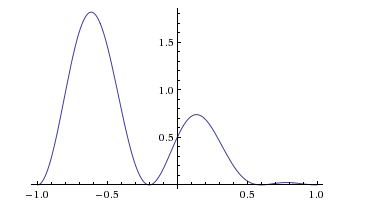
\includegraphics{mixed_states.png}
\caption{Probability density function of super position of first and second excited states.}
\label{fig:mixed_states}
\end{figure}
\end{subsubanswer}

\begin{subsubanswer}
We can calculate the average value of the position operator directly, calculating it as follows:
\begin{align*}
\langle x \rangle &= \int_{-a/2}^{a/2} x |\Psi(x,t)|^2 dx \\
&= \frac{1}{a} [ \underbrace{\int_{-a/2}^{a/2} x \sin^2\left(\frac{2\pi}{a}x \right) dx}_{\text{=0 because it is odd}} + \underbrace{\int_{-a/2}^{a/2} x \cos^2\left(\frac{3\pi}{a}x\right)dx}_{\text{=0 because it is odd}} \\
&+ \left[e^{-i[E_3 - E_2]t / \hbar} + e^{i[E_3-E_2]t / \hbar} \right]\underbrace{\int_{-a/2}^{a/2} x \sin\left(\frac{2\pi}{a}x \right)\cos\left(\frac{3\pi}{a}x \right) dx}_{\text{constant}} ] \\
&= \underbrace{2\cos[(E_3 - E_2)t]}_{\text{by euler}}\underbrace{\int_{-a/2}^{a/2} x \sin\left(\frac{2\pi}{a}x \right)\cos\left(\frac{3\pi}{a}x \right) dx}_{\text{=A, a constant}} \\
&=
\underbrace{2A\cos\left(\frac{5\hbar^2\pi^2}{2ma^2}t \right)}_{\text{using definition of }E_n}
\end{align*}
\end{subsubanswer}

\begin{subsubanswer}
We can see in Figure \ref{fig:mixed_states} the probability for $t=0$. Note that given the equations above, we have a constant contribution which consists of simply mixing the two stationary distributions.
$$
\frac{1}{a}\left[ \sin^2\left(\frac{2\pi}{a}x \right) + \cos^2\left(\frac{3\pi}{a}x \right) \right]
$$
However, we also have a factor which depends on time given by:
$$
\frac{2}{a}\cos[(\frac{5\hbar \pi^2}{2ma^2})t]\sin\left(\frac{2\pi}{a}x \right) \cos\left(\frac{3\pi}{a}x \right)
$$
Due to the cosine factor, this wave is cyclic with period $t= \frac{4ma^2}{5\hbar \pi}$, at which point it returns to the shape seen in Figure \ref{fig:mixed_states}. How about in between? If we input $t = \frac{2ma^2}{5\hbar\pi}$ we obtain the reverse of the shape shown in Figure \ref{fig:mixed_states} (we see this in Figure \ref{fig:mixed_states_2}.
\begin{figure}[h!]
\centering
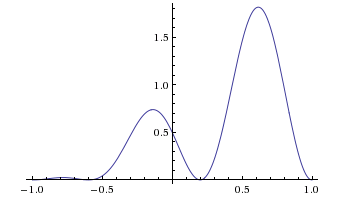
\includegraphics{mixed_states_2.png}
\caption{The probability density function of the super position of first and second excited states at $t = \frac{2ma^2}{5\hbar\pi}$.}
\label{fig:mixed_states_2}
\end{figure}
As we can tell from the figures, the particle seems to be bouncing inside the box from the left to the right and will continue to do so.
\end{subsubanswer}

\begin{subsubanswer}
As we can see from the results above, the average position oscillates as time passes. Intuitively, what's going on is that the wave is moving from the stationary shape shown in Figure \ref{fig:mixed_states} at $t= 0$ to the right as shown in Figure \ref{fig:mixed_states_2} and then bouncing back to the same in Figure \ref{fig:mixed_states}. Therefore, the average position does the same. We arbitrarily set $A = \frac{1}{2}$ as we only care about the shape of the graph (not the amplitude), and we note that as time passes, we have the average position operator do something like that shown in Figure \ref{fig:position_operator}, with a period length of $\frac{4ma^2}{2\hbar^2\pi}$.
\begin{figure}
\centering
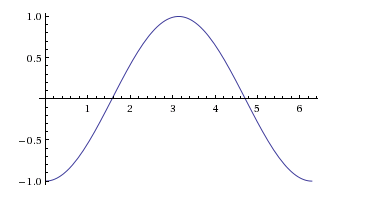
\includegraphics{cosine.png}
\caption{Just a simple cosine graph, which is the expected behaviour of the average position operator}
\label{fig:position_operator}
\end{figure}
\end{subsubanswer}

\begin{subsubanswer}
Now we tackle the momentum operator. By definition we have:
\begin{align*}
\langle p \rangle &= \int_{-a/2}^{a/2} \Psi^*(x,t) \hat{p} \Psi(x,t) dx \\
&= \underbrace{\frac{1}{2}\int_{-a/2}^{a/2} \Psi_2^*(x,t) \hat{p} \Psi_2(x,t) dx}_{\text{=0, average momentum operator for $\Psi_2$}} + \underbrace{\frac{1}{2}\int_{-a/2}^{a/2} \Psi_3^*(x,t) \hat{p} \Psi_3(x,t) dx}_{\text{=0, average momentum operator for $\Psi_3$}} \\
&+\frac{1}{2}\left[\int_{-a/2}^{a/2} \Psi^*_3(x,t)\hat{p}\Psi_2(x,t) dx + \int_{-a/2}^{a/2} \Psi^*_2(x,t) \hat{p} \Psi_3(x,t) dx \right] \\
&= -\frac{i\hbar}{2}\left[\int_{-a/2}^{a/2} \Psi^*_3(x,t)\frac{\partial}{\partial x}\Psi_2(x,t) dx + \int_{-a/2}^{a/2} \Psi^*_2(x,t) \frac{\partial}{\partial x} \Psi_3(x,t) dx \right]\\
&= -\frac{i \hbar}{2} \left[\frac{4\pi}{a^2} e^{i[E_3-E_2]t / \hbar} \underbrace{\int_{-a/2}^{a/2} \cos(\frac{3\pi}{a}x)\cos(\frac{2\pi}{a}x)dx}_{\text{constant}}   - \frac{6\pi}{a^2}e^{-i[E_3 - E_2]t /\hbar} \underbrace{\int_{-a/2}^{a/2} \sin(\frac{3\pi}{a}x)\sin(\frac{2\pi}{a}x) dx}_{\text{constant}} \right] \\
&= \beta_1e^{i[E_3 - E_2]t / \hbar} - \beta_2 e^{-i[E_3 -E_2]t / \hbar}
\end{align*}
For reference, see Griffith. As we can see, the momentum operator depends on time in a wave-like fashion. As $t$ passes, the momentum oscillates from positive to negative and then back, similar to the position. A sketch is provided in Figure \ref{fig:sketch_3}:

\begin{figure}[h!]
\centering

\includegraphics{blank.png}
\caption{Sketch of Momentum Operator Change with Time}
\label{fig:sketch_3}
\end{figure}

\end{subsubanswer}
\end{subanswer}
\end{answer}

\begin{answer}
We tackle the infinite square well potential once again with the initial wave function given by $\Psi(x,t) = Ax(a - x)$.

\begin{subanswer}
We have the following wave function at time $t = 0$:
$$
\Psi(x) = \Psi(x,0) = Ax(a - x)
$$
Note that if we normalize $\Psi(x)$, then $\Psi(x,t)$ will stayed normalized (as shown in a previous homework assignment). Then we have:
\begin{align*}
\int_0^a |\Psi(x,0)|^2 dx &= A^2 \int_0^a x^2(a-x)^2 dx \\
&= A^2\int_0^a a^2x^2 + x^4 -2ax^3 dx \\
&= A^2\left[\frac{a^2}{3}x^3 + \frac{1}{5}x^5 - \frac{a}{2}x^4 \big|_0^a\right] \\
&= A^2a^5\left(\frac{1}{3} + \frac{1}{5} - \frac{1}{2} \right) \\
&= A^2\frac{a^5}{30}
\end{align*}
Therefore we need to have:
$A = \sqrt{\frac{30}{a^5}}$

as the normalization constant. The plot is given in Figure \ref{fig:initial_condition} for $a = 1$.

\begin{figure}[h!]
\centering
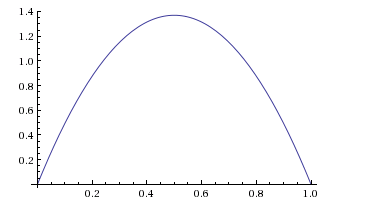
\includegraphics{initial_condition.png}
\caption{Initial condition for wave function.}
\label{fig:initial_condition}
\end{figure}
\end{subanswer}

\begin{subanswer}
The plot most closely resembles the stationary state for $n = 1$ given by:
$$
\Psi_1(x) = \sqrt{\frac{2}{\alpha}}\sin\left(\frac{\pi}{a}x \right)
$$
which means that we'd estimate the energy to be $E_1 = \frac{\hbar^2 \pi^2}{2ma^2}$.
\end{subanswer}

\begin{subanswer}
We now compute the average value of the position operator. We do this directly on the wave function $\Psi(x,t) = Ax(a-x)$.
\begin{align*}
\langle x \rangle &= \int_{0}^a x |\Psi(x,t)|^2 dx \\
&= \frac{30}{a^5}\int_0^a x^3(a-x)^2 dx \\
&= \frac{30}{a^5}\int_0^a a^2x^3 - 2ax^4 + x^5 \\
&= \frac{30}{a^5} \left[ \frac{1}{4}a^2x^4 - \frac{2}{5}ax^5 + \frac{1}{6}x^6 \biggr|_0^a\right] \\
&= \frac{30a}[\frac{1}{4} - \frac{2}{5} + \frac{1}{6}] \\
&= \frac{a}{20}
\end{align*}
\end{subanswer}

\begin{subanswer}
We now calculate the expected value of the linear momentum operator. We expect the result to be $0$.
\begin{align*}
\langle p \rangle &= \int_0^a \Psi^* \hat{p} \Psi dx \\
&= -i\hbar A^2 \int_0^a x(a-x) \frac{d}{dx}[x(a-x)] dx \\
&= -i\hbar A^2 \int_0^a x(a-x)(a-2x) dx \\
&= -i\hbar A^2 \int_0^a a^2x + 2x^3 - 3ax^2 dx \\
&= -i\hbar A^2 \left[\frac{1}{2}a^2x^2 + \frac{1}{2}x^4 - ax^3 \biggr|_0^a \right] \\
&= -i\hbar A^2a^4(\frac{1}{2} + \frac{1}{2} - 1) \\
&= 0
\end{align*}
\end{subanswer}

\begin{subanswer}
We now calculate the ensemble average of the total energy operator. We assume no potential.
\begin{align*}
\langle H \rangle &= \int_0^a \Psi^*(-\frac{\hbar^2}{2m}\frac{\partial^2}{\partial x^2})\Psi dx \\
&= \frac{A^2\hbar^2}{m}\int_0^a x(a-x) dx \\
&= \frac{A^2\hbar^2}{m}\left[\frac{a}{2}x^2 - \frac{1}{3}x^3 \biggr|_0^a \right] \\
&= \frac{5\hbar^2}{ma^2}
\end{align*}
Note that the above agrees closely with what we would expect for the ground state, given by $\frac{\hbar^2\pi^2}{2ma^2}$. Note that the ratio is:
$$
\frac{10}{\pi^2} \approx 1
$$
which is pretty darn good!
\end{subanswer}

\begin{subanswer}
We can write our initial wave function as:
$$
\Psi(x,0) = \sum_{i=1}^{\infty} c_n \Psi_n(x)
$$
We know from lecture that we can use the trick of multiplying by $\Psi_n$ to kill off all the other $\Psi_m$ where $m \neq n$. This gives us the following formula for the $c_n$:
\begin{align*}
c_n &= \int_0^a \Psi_n^*(x)\Psi(x,0)dx \\
&=
\end{align*}
\end{subanswer}
\end{answer}

\begin{answer}
We create a potential with the following form:
$$
V(x) = \begin{cases}
V_0 & x < -a \\
0 & |x| < a \\
3V_0 & x > a
\end{cases}
$$
where $V_0 > 0$.

\begin{subanswer}
A plot is shown in Figure \ref{fig:potential_landascape}.

\begin{figure}[h!]
\centering
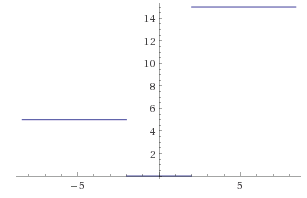
\includegraphics{potential.png}
\caption{Potential Landspace instantiated with $a = 2$ and $V_0 = 5$. General shape is similar.}
\label{fig:potential_landascape}
\end{figure}
\end{subanswer}

\begin{subanswer}
For energy states between $0$ and $V_0$, a sketch of the a possible eigenstate is shown in Figure \ref{fig:potential_landascape}. The points to note are that the exponentials on each side decay at different rates, with the exponential on the $3V_0$ side decaying faster.
\end{subanswer}

\begin{subanswer}
The solutions must take the following analytic forms. As labeled in Figure \ref{fig:potential_landascape}, for Region $I$:
$$
\Psi_I(x) = \underbrace{Ae^{-k_1x}}_{\text{A = 0}} + Be^{k_1x}
$$
where the first term is $0$ to prevent exponential blow-up as $x \to -\infty$ since $k > 0$ with $k_1 = \frac{1}{\hbar}\sqrt{2m(V_0 - E)}$. Similarly, for Region III:
$$
\Psi_{III}(x) = Ee^{-k_2x} + \underbrace{Fe^{k_2x}}_{\text{F = 0}}
$$
where again the second term is $0$ to prevent exponential blow-up as $x \to \infty$. For both of the cases above, we have $k_2 = \frac{1}{\hbar}\sqrt{2m(3V_0 - E)}$ where $E$ is the energy of this eigenstate.

And lastly, for region $II$, we have:
$$
\Psi_{II}(x) = C\sin lx + D \cos lx
$$
where $l = \frac{1}{\hbar}\sqrt{2mE}$.
\end{subanswer}

\begin{subanswer}
Now we apply the matching condition for our solutions. Note that we require the wave-function to be continuous and its derivative to be continous, which leads to the following set of equations:
\begin{align*}
Be^{-k_1a} = -C \sin la + D \cos la \tag{continuity of $\Psi$ at $x = -a$} \\
C \sin la + D \cos la = Ee^{-k_2a} \tag{continuity of $\Psi$ at $x = a$} \\
k_1Be^{-k_1a} = lC\cos la + lD \sin la \tag{continuity of $\Psi'$ at $x = - a$} \\
lC\cos la - lD \sin la = -k_2E^{-k_2a} \tag{continuity of $\Psi'$ at $x = a$}
\end{align*}
The above are the sets of equations that we would like to solve. Note that we have four unknowns ($B,C,D$ and $E$) and four equations, so we should be able
to solve (if not analytically, then numerically).
\end{subanswer}

\begin{subanswer}
For energy states between $V_0$ and $3V_0$, a sketch of the a possible eigenstate is shown in Figure \ref{fig:potential_landascape}. The point to note is that the exponential decays off in Region $III$ and that the amplitude and wavelength are somewhat smaller in Region $II$ as compared to Region $I$.
\end{subanswer}

\begin{subanswer}
The solutions must take the following analytic form. As labeled in Figure \ref{fig:potential_landascape}, for Region $I$:
$$
\Psi_I(x) = A\sin l_1x + B\cos l_1x
$$
where $l_1 = \frac{1}{\hbar}\sqrt{2m(E-V_0)}$. Similarly for Region $II$:
$$
\Psi_{II}(x) = C \sin l_2x + D \cos l_3 x
$$
where $l_2 = \frac{1}{\hbar}\sqrt{2mE}$, and lastly, for Region $III$:
$$
\Psi_{III}(x) = Ee^{-kx} + \underbrace{Fe^{kx}}_{F = 0}
$$
where the second term is $0$ to prevent exponential blow-up as $x \to \infty$ and $k = \frac{1}{\hbar}\sqrt{2m(3V_0 - E)}$.
\end{subanswer}

\begin{subanswer}
Now we apply the matching condition for our solutions. Note that we require the wave-function to be continuous and its derivative to be continuous, which leads to the following set of equations:
\begin{align*}
-A \sin l_1a + B \cos l_1 x = -C \sin l_2a + D \cos l_2a \tag{continuity of $\Psi$ at $x = -a$} \\
C \sin l_2a + D \cos l_2a = Ee^{-ka} \tag{continuity of $\Psi$ at $x = a$} \\
l_1A\cos l_1a + l_2B l_1a = l_2C\cos l_2a + l_2D \sin l_2a \tag{continuity of $\Psi'$ at $x = - a$} \\
l_2C\cos l_2a - l_2D \sin l_2a = -kE^{-ka} \tag{continuity of $\Psi'$ at $x = a$}
\end{align*}
The above are the sets of equations that we would like to solve. Note that we have five unknowns ($A, B,C,D$ and $E$) and four equations, so we should be able to solve (if not analytically, then numerically) using the additional fact that the wave function must be normalized.
\end{subanswer}

\begin{subanswer}
For energy states above $3V_0$, a sketch of the a possible eigenstate is shown in Figure \ref{fig:potential_landascape}. The point to note is that the amplitude and wavelength are somewhat smaller in Region $II$ as compared to Region $I$ as compared to Region $III$.
\end{subanswer}

\begin{subanswer}
The solutions must take the following analytic form. As labeled in Figure \ref{fig:potential_landascape}, for Region $I$:
$$
\Psi_I(x) = A\sin l_1x + B\cos l_1x
$$
where $l_1 = \frac{1}{\hbar}\sqrt{2m(E-V_0)}$. Similarly for Region $II$:
$$
\Psi_{II}(x) = C \sin l_2x + D \cos l_3 x
$$
where $l_2 = \frac{1}{\hbar}\sqrt{2mE}$, and lastly, for Region $III$:
$$
\Psi_{III}(x) = E \sin l_3x + F \cos l_3 x
$$
where $l_3 = \frac{1}{\hbar}\sqrt{2m(E - 3V_0)}$.
\end{subanswer}

\begin{subanswer}
Now we apply the matching condition for our solutions. Note that we require the wave-function to be continuous and its derivative to be continuous, which leads to the following set of equations:
\begin{align*}
-A \sin l_1a + B \cos l_1 x = -C \sin l_2a + D \cos l_2a \tag{continuity of $\Psi$ at $x = -a$} \\
C \sin l_2a + D \cos l_2a = E \sin l_2a + F \cos l_2a \tag{continuity of $\Psi$ at $x = a$} \\
l_1A\cos l_1a + l_2B l_1a = l_2C\cos l_2a + l_2D \sin l_2a \tag{continuity of $\Psi'$ at $x = - a$} \\
l_2C\cos l_2a - l_2D \sin l_2a = -l_3E\cos l_3a - l_2F \sin l_2a \tag{continuity of $\Psi'$ at $x = a$}
\end{align*}
The above are the sets of equations that we would like to solve. Note that we have five unknowns ($A, B,C,D$ and $E$) and four equations, so we should be able to solve (if not analytically, then numerically) using the additional fact that the wave function must be normalized.
\end{subanswer}

\begin{subanswer}
In order to solve any of the above problems, we would simply need to do some algebra. Note that for each of the regions with the boundary conditions we have sufficient equations and restraints to solve for the coefficients as required. There are multiple sources online and in the textbook that take advantage of this, so I would suggest taking a look over those before solving completely. Note that some of the solutions are unlikely to be analytical (as was the case with the symmetric well), and instead it would be required to use some sort of equation solver package. In that scenario, we should be able to approximate the coefficients to as close a result as possible.

The next step after solving for the coefficients which lets use solve for the eigenstates is to then express the initial state and the initial conditions as a linear combination of these determined states. We then use the normal tricks to calculate the weight $|c_i|^2$ of each function.
\end{subanswer}

\end{answer}

\begin{answer}
Note that we're considering obtaining the energy eigenvalues and eigenfunctions for an infinite square well by taking the limit of a finite square well. Then note that we can assume the finite square well to be symmetric, as the infinite square well is symmetry. We center the well so that it has width $2a$ and height $V_0 > 0$ as follows:
$$
V(x) = \begin{cases}
-V_0 & |x| < a \\
0 & \text{ otherwise}
\end{cases}
$$
Furthermore, note that in the limit, all states are bounded. Therefore, we only consider what occurs to the bounded states of the finite square well. We did this in section, in lecture, and is in the textbook, but for a refresher on notation, we summarize the results once again. First, in each region, the general solution to the SE looks like the following:
\begin{align*}
\Psi_I(x) &= Ae^{kx} \tag{Region I} \\
\Psi_{II}(x)&= C\cos lx + D \sin lx \tag{Region II} \\
\Psi_{III}(x) &= Fe^{-kx} \tag{Region III}
\end{align*}
where $k = \frac{1}{\hbar}\sqrt{2mE}$ and $l = \frac{1}{\hbar}\sqrt{2m(V_0 + E)}$. The above are the only physically admissible solutions in order to allow the wave function to be normalizable.

Next we impose the boundary conditions. Note that due to the parity of the potential, the solution will either be odd or even. We tackle each approach separately and take their limits separately.

First, we begin with the even solutions as covered in the textbook. Imposing boundary conditions we have:
\begin{align*}
Fe^{-ka} &= C \cos(la) \tag{$\Psi$ continuous at $x=a$} \\
-kFe^{-ka} &= -lC \sin(la) \tag{$\Psi'$ continuous at $x = a$}
\end{align*}
Dividing, we have $k = l \tan(la)$.
We now let $z \equiv la$ and $z_0 \equiv \frac{a}{\hbar}\sqrt{2mV_0}$. Note that $k^2 + l^2 = 2mV_0/\hbar^2$, therefore $ka = \sqrt{z_0^2 - z^2}$, which gives use the solution:
$$
\tan z = \sqrt{\left(\frac{z_0}{z}\right)^2 - 1}
$$
We can solve the above for $z_n$ and subsequently get $E_n$ (note this is only for $n$ odd, since we're only considering the odd functions at the moment). Then note that as $V_0 \to \infty$, we have $z_0 \to \infty$ and $\sqrt{\left(\frac{z_0}{z}\right)^2 - 1} \to \infty$. This means that $z_n \approx \frac{n\pi}{2}$ for odd $n$ since this is when $\tan z_n$ diverges. The we have:
$$
z_n = la = \frac{1}{\hbar} \sqrt{2ma(E_n+V_0)}\implies E_n + V_0 = \frac{z_n^2\hbar^2}{2ma} = \frac{n^2\pi^2\hbar^2}{2m(2a)^2}
$$
Then note that $E + V_0$ is precisely the energy above the bottom of the well, so we actually have an approximation of the infinite square well where we've started the well at the x-axis and the walls extend upward (rather than the way we approached it originally, were we make the well deeper).

We can now repeat the process for the odd solutions. We have the same boundary conditions but with $D = 0$ instead of $C=0$ (so that we only consider $\sin(lx)$), and through the same process as above, we obtain $k = \cot(la)$, and letting $z,z_0$ be as defined above, we have:
$$
\cot z = \sqrt{\left(\frac{z_0}{z} \right)^2 - 1}
$$
For large $V_0$, we have $z_n \approx \frac{n\pi}{2}$ for even $n$ since this is when $\sin$ vanishes. Then we have:
$$
z_n = la = \frac{1}{\hbar}\sqrt{2ma(E_n + V_0)} \implies E_n + V_0 = \frac{z_n^2\hbar^2}{2ma} = \frac{n^2\pi^2\hbar^2}{2m(2a)^2}
$$
Then by similar logic to the above, these are actually the energies for the infinite square well for the even states!
\end{answer}

\begin{answer}
We have a particle in a well with width $w$ and depth $V_0$. Now we consider the case where $w \to 0$ and $V_0 \to \infty$ yet $wV_0 \to a$ for some finite $\alpha$. Note that this is the same as having a Delta-Function Potential given by:
$$
V(x) = -\alpha\delta(x)
$$
We therefore follow Griffith carefully.

\begin{subanswer}
We begin by looking for bounded states. Note that $\Psi$ will take the form:
$$
\Psi_I(x) = Ae^{kx}
$$
for $x < 0$ and
$$
\Psi_{III}(x) = A^{-kx}
$$
for $x > 0$ where $k = \frac{1}{\hbar}\sqrt{-2mE}$. Note that due to the continuity of $\Psi$, the coefficients had to be same. We have thusfar gathered no further information, but in the spirit of Griffith, we now integrate the SE from $-\epsilon$ to $\epsilon$ and then take the limit as $\epsilon \to 0$:
$$
-\frac{\hbar^2}{2m} \int_{-\epsilon}^{\epsilon} \frac{\partial^2}{\partial x^2} \Psi dx - \alpha \int_{-\epsilon}^{\epsilon} \delta(x)\Psi(x) dx = E\int_{-\epsilon}^{\epsilon} \Psi(x) dx
$$
The RHS goes to $0$, as we're integrating a function with an absolute maximum ($\Psi(0) = A$) over an infinitely small region. The first term on the LHS is straight forward to evaluate:
$$
-\frac{\hbar^2}{2m} \int_{-\epsilon}^{\epsilon} \frac{\partial^2}{\partial x^2} \Psi(x) dx = -\frac{\hbar^2}{2m}\left[\frac{\partial \Psi}{\partial x} \biggr|_{-\epsilon}^{\epsilon} \right]
$$
For the middle term, note that by definition of the delta function, as $\epsilon \to 0$, we have:
$$
\alpha\int_{-\epsilon}^{\epsilon} \delta(x)\Psi(x)dx = \alpha\Psi(0) = \alpha A
$$
Then looking at the one-sided derivatives, we also have that:
\begin{align*}
\lim_{x \to 0^+} \frac{\partial \Psi(x)}{\partial x} &= \lim_{x \to 0^+} -kAe^{-kx} = -kA \\
\lim_{x \to 0^-} \frac{\partial \Psi(x)}{\partial x} &= \lim_{x \to 0^-} kAe^{kx} = kA
\end{align*}
This give us, for $\epsilon \to 0$
$$
-\frac{\hbar^2}{2m}\left[\frac{\partial \Psi}{\partial x}\biggr|_{-\epsilon}^{\epsilon} \right] = -\frac{\hbar^2}{2m}[-kA - kA] = \frac{\hbar^2 kA}{m}
$$
Then this implies that:
\begin{align*}
\frac{\hbar^2kA}{m} = \alpha A \implies k = \frac{m \alpha}{\hbar^2}
\end{align*}
This gives allowed energy given by:
$$
E = -\frac{\hbar^2 k^2}{2m} = -\frac{m\alpha^2}{2\hbar^2}
$$
Finally, we can normalize the wave function:
\begin{align*}
\int_{\infty}^{\infty} |\Psi(x)|^2 &= 2|B|^2 \int_0^\infty e^{-2kx} dx \\
&= \frac{|B|^2}{k} = 1 \\
\implies B &= \sqrt{k} = \frac{\sqrt{ma}}{\hbar}
\end{align*}
Therefore, by the above, we arrive at exactly one bound state given by:
$$
\Psi(x) = \frac{\sqrt{ma}}{\hbar}e^{-\frac{ma}{\hbar^2}|x|}
$$
and bound energy:
$$
E = -\frac{ma^2}{2\hbar^2}
$$
\end{subanswer}

\begin{subanswer}
We now consider the unbound (continuum) states. Following the same formula as before, we note that in Region $I$ the wave function takes on the form:
$$
\Psi_I(x) = Ae^{ikx} + B e^{-ikx}
$$
and for Region $III$:
$$
\Psi_{III}(x) = Ee^{ikx} + F e^{-ikx}
$$
Then continuity at $x = 0$ forces:
$$
A + B = E +F
$$
and the boundary derivative:
\begin{align*}
\lim_{x\to 0^+} \frac{\partial}{\partial x}\Psi(x) = ik(F-G) \\
\lim_{x\to 0^-} \frac{\partial}{\partial x}\Psi(x) = ik(A-B)
\end{align*}
and hence the difference is $ik(F - G - A + B)$, while $\Psi(0) = A + B$, so that by the second boundary condition:
$$
ik(F - G - A + B) = -\frac{2ma}{\hbar^2}[A + B]
$$
or more compactly:
$$
F-G = A(1 + 2i\beta) - B(1 - 2i\beta)
$$
where $\beta = \frac{ma}{\hbar^2 k}$. At this point, note that we do not have enough information to solve for these constants, so we leave it to the wind :)

On another note, for a more thorough explanation, please see Griffith's presentation. In it, he explores the behavior of these free states.

\end{subanswer}
\end{answer}

\begin{answer}
15 hours!
\end{answer}

\begin{answer}
Keep up the great work!
\end{answer}
\end{document}